\documentclass[c]{beamer}
\usetheme{default}
\title{Generalizing Nondeterminism for Algebraic Computation Machines}
\author{Scott Sanderson}
\institute{Department of Mathematics\\Williams College}
\date{\today}
\usepackage{tikz}
\usepackage{beamerthesiscommands}
\usepackage{mydiagrams}
\usepackage{graphicx}
\usepackage{algorithm}
\usepackage{algorithmicx}
\usepackage{algpseudocode}
\renewcommand{\algorithmicrequire}{\textbf{Input:}}
% \usepackage{enumitem}
\usetikzlibrary{calc,arrows,shapes,positioning}

\begin{document}

\theoremstyle{definition}
\newtheorem{proposition}{Proposition}
\newtheorem{proofidea}{Proof Idea}

% \begin{frame}
%   \titlepage
% \end{frame}

% \begin{frame}{Computability and Complexity Theory}
  
%   \begin{columns}
%     \visible<1->{
%       \column{0.5\textwidth}
%       \begin{figure}[h]
%         \centering \scaletopagewidth{\algoyesno{}}
%       \end{figure}
%     }
%     \visible<2->{
%       \column{0.6\textwidth}
%       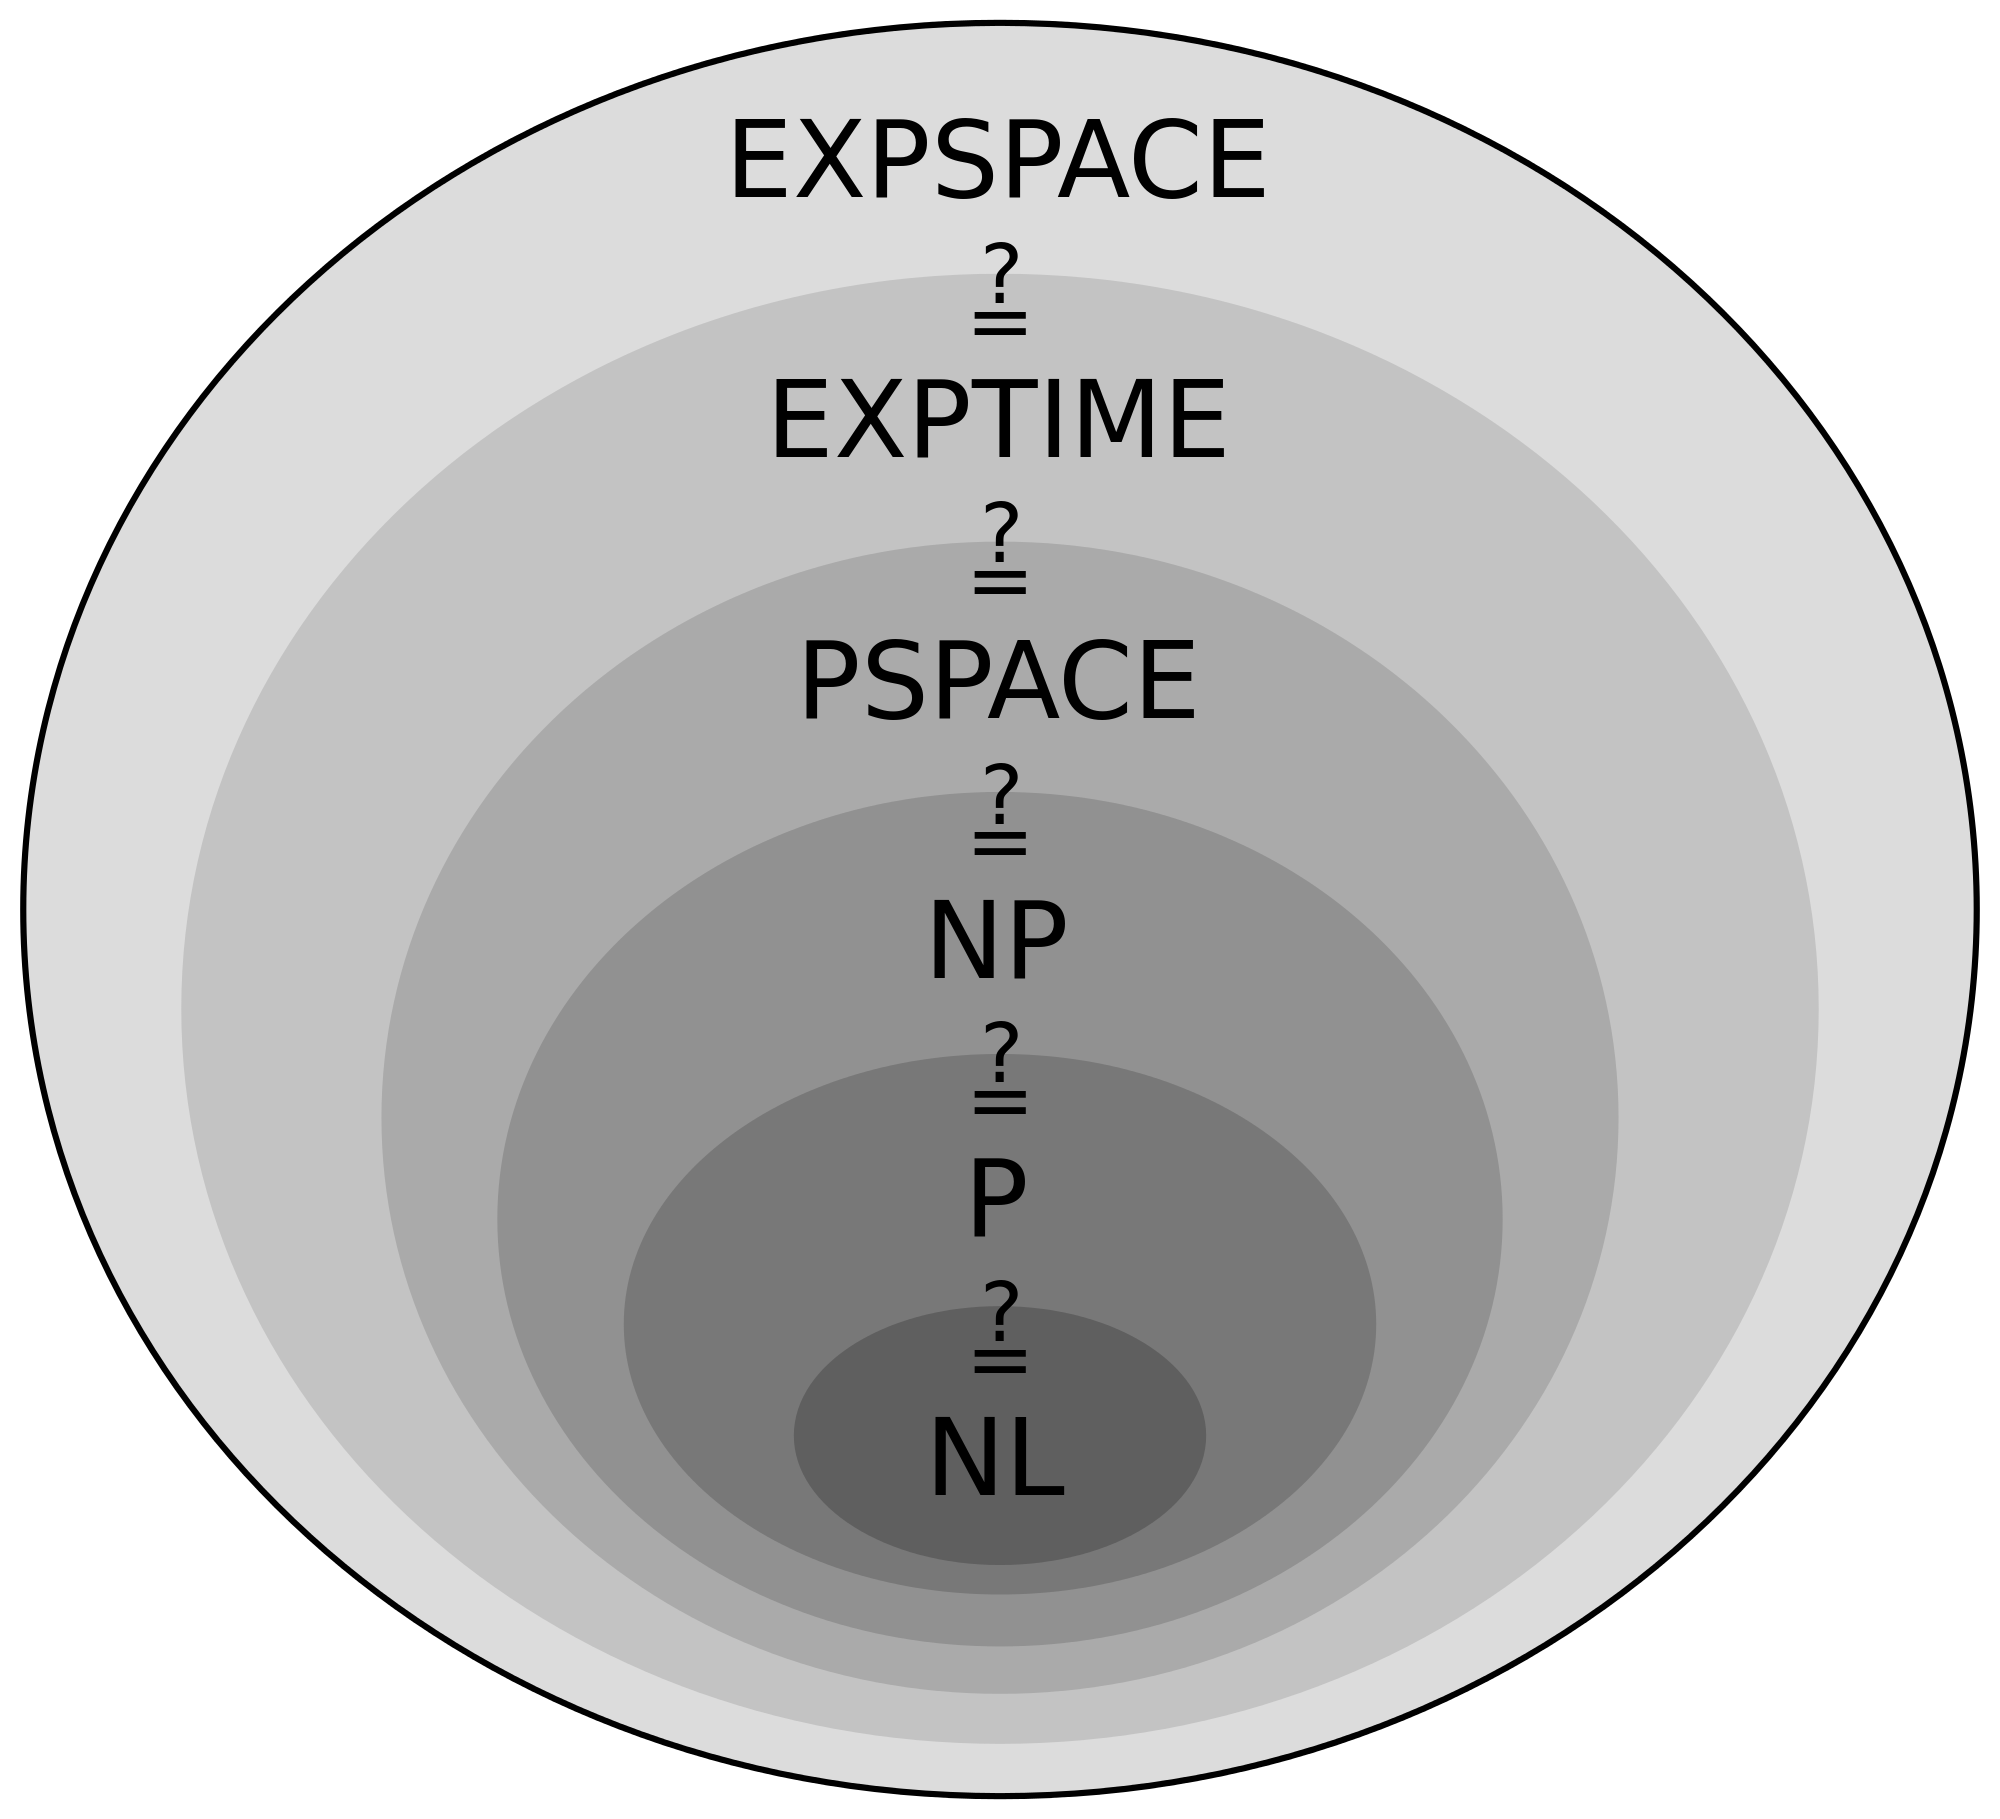
\includegraphics[width=\textwidth]{media/complexity.png}    
%     }
%   \end{columns}

% \end{frame}

% \begin{frame}{Outline}
%   \begin{center}
%     \scaletopagewidth{\outlinenobss}
%   \end{center}
% \end{frame}

% \begin{frame}{Outline}
%   \begin{center}
%     \scaletopagewidth{\outlinenondet}
%   \end{center}
% \end{frame}

% \begin{frame}{Outline}
%   \begin{center}
%     \scaletopagewidth{\outlinealmostfinal}
%   \end{center}
% \end{frame}

% \begin{frame}{Outline}
%   \begin{center}
%     \scaletopagewidth{\outlinefinal}
%   \end{center}
% \end{frame}

% \begin{frame}{A Simple Puzzle}
  
%   \begin{itemize}
%   \item[] Does the set: $\set{1,4,7,-5,-3,18,-6,12}$ contain
%     a subset adding up to 10? \pause
%   \item[] Yes.  \textbf{Proof}: $18 - 3 - 6 + 1 = 10$ \pause
%   \item[] Does $\set{1, 17, 25, -3, 11, -9, 22, 13}$ contain a subset
%     adding up to 7?\pause
%   \item[] No.  \textbf{Proof}: Err...try them all? 
%   \end{itemize}
  
% \end{frame}

% \begin{frame}{\subsum{}}

%   An \textbf{instance} of \subsum{} is a pair $(S, t)$, where:

%     \begin{itemize}
%     \item $S = \set{s_1, s_2, \ldots, s_n}$ is a set of integers.
%     \item $t$ is a single integer, called the \textbf{target} for $S$.
%     \end{itemize}\pause

%     \vspace{\baselineskip}

%     An instance of \subsum{} is a \textbf{Yes Instance} if
%     there exists some $X \subseteq S$ such that $\sum_X = t$.

%     \vspace{\baselineskip}
    
%     Otherwise it is a \textbf{No Instance}.
% \end{frame}

% \begin{frame}{Decision Problems}

%   \begin{itemize}
%   \item[] \subsum{} is an example of a \textbf{Decision Problem}.\pause

%     \vspace{\baselineskip}

%   \item[] A Decision Problem $D$ is a set of values, partitioned into
%     Yes Instances and No Instances, $D_{yes}$ and $D_{no}$.

%   \item[] Goal is to find an algorithm that ``accepts'' $D_{yes}$ and
%     ``rejects'' $D_{no}$.  Such an algorithm \textbf{decides} $D$.
%   \end{itemize}

% \end{frame}

% \begin{frame}{Classical Machine Model - Turing Machines}
%   \begin{columns}

%     \column{0.5\textwidth}
%     \begin{itemize}
%     \item[] Infinite one-way tape, divided into cells.    
%     \end{itemize}
%     \column{0.5\textwidth}
%     \scaletopagewidth{\tape{$q$}{{1,0,1,0,0,$\blank$, $\blank$, $\cdots$}}}
%   \end{columns}
% \end{frame}

% \begin{frame}{Classical Machine Model - Turing Machines}
%   \begin{columns}

%     \column{0.5\textwidth}
%     \begin{itemize}
%     \item At each step, tape head reads a symbol, writes a symbol,
%       moves left/right, and changes state.
%     \end{itemize}
    
%     \column{0.5\textwidth}
%     \scaletopagewidth{\tape[1]{$q$}{{1,0,1,0,0,$\blank$, $\blank$, $\cdots$}}}
%     $$\delta(q, 1) = (q', 0, \rightarrow)$$
%     \scaletopagewidth{\tape[2]{$q'$}{{0,0,1,0,0,$\blank$, $\blank$, $\cdots$}}}
%   \end{columns}
% \end{frame}

% \begin{frame}{Turing Machines}
%   \begin{columns}

%     \column{0.5\textwidth}
%     \begin{itemize}
%     \item Computation ends when we enter special states $q_{accept}$
%       or $q_{reject}$.
%     \end{itemize}
%     \column{0.5\textwidth}
%     \scaletopagewidth{\tape[3]{$q'$}{{0,1,1,0,0,$\blank$, $\blank$, $\cdots$}}}
%     $$\delta(q', 1) = (q_{acc}, 1, \leftarrow)$$
%     \scaletopagewidth{\tape[2]{$q_{acc}$}{{0,1,1,0,0,$\blank$, $\blank$, $\cdots$}}}
%   \end{columns}
% \end{frame}

% \begin{frame}{Turing Machine Example - Even or Odd?}
%   \begin{columns}[c]
    
%     \small

%     \column{0.5\textwidth}

%     \begin{itemize}
%     \item[] $Q = \set{q_0, q_1, q_{acc}, q_{rej}}$
%     \item[] $\Gamma = \set{\blank, 0, 1}$
%     \item[] $\Sigma = \set{0,1}$
%     \item[] $\delta(q_0, 0) = (q_0, \blank, \rightarrow)$
%     \item[] $\delta(q_0, 1) = (q_1, \blank, \rightarrow)$
%     \item[] $\delta(q_0, \blank) = (q_{acc}, \blank, \leftarrow)$
%     \item[] $\delta(q_1, 0) = (q_0, \blank, \rightarrow)$
%     \item[] $\delta(q_1, 1) = (q_1, \blank, \rightarrow)$
%     \item[] $\delta(q_1, \blank) = (q_{rej}, \blank, \leftarrow)$
%     \end{itemize}

%     \column{0.5\textwidth}
    
%       \scaletopagewidth[0.8]{\tape[1]{$q_0$}{{1,0,1,0,$\blank$,$\cdots$}} \vspace{1mm}}
%       \scaletopagewidth[0.8]{\tape[2]{$q_1$}{{$\blank$,0,1,0,$\blank$,$\cdots$}} \vspace{1mm}}
%       \scaletopagewidth[0.8]{\tape[3]{$q_0$}{{$\blank$,$\blank$,1,0,$\blank$,$\cdots$}} \vspace{1mm}}
%       \scaletopagewidth[0.8]{\tape[4]{$q_1$}{{$\blank$,$\blank$,$\blank$,0,$\blank$,$\cdots$}} \vspace{1mm}}
%       \scaletopagewidth[0.8]{\tape[5]{$q_0$}{{$\blank$,$\blank$,$\blank$,$\blank$,$\blank$,$\cdots$}} \vspace{1mm}}
%       \scaletopagewidth[0.8]{\tape[4]{$q_{acc}$}{{$\blank$,$\blank$,$\blank$,$\blank$,$\blank$, $\cdots$}} \vspace{1mm}}
      
%   \end{columns}
% \end{frame}

% \begin{frame}{\subsum{} Generalized}
  
%   \begin{itemize}
%   \item[] Does the set $\set{1,\frac{3}{4},\sqrt{2},-5,-3,18,-6,12}$
%     contain a subset adding up to $\pi$?
%   \end{itemize}
% \end{frame}

% \begin{frame}{The Mandelbrot Set $\mathcal{M}$}
  
%   Let $c \in \complexes$, we define:
%     \begin{align*}
%       p_c(z) &= z^2 + c\\
%       p_c^n(z) &= p_c(\ldots(p_c(p_c(z)))) \text{ $n$ times }\\
%     \end{align*}
    
%     \vspace{-\baselineskip}
    
%     The Mandelbrot Set $\mathcal{M}$ is given by:
%     $$\set{c \in \complexes |p_c^n(0) \nrightarrow \infty \text{ as } n \rightarrow \infty}$$
    
% \end{frame}

% \begin{frame}{The Mandelbrot Set $\mathcal{M}$}

%   
\includegraphics[width=\textwidth]{media/mandelbrot.jpg}
  
% \end{frame}

% \begin{frame}{The Mandelbrot Set as Decision Problem}
  
%   \begin{itemize}
%   \item[] ``Easy'' to tell if $c \in \complexes$ is \textbf{not} in
%     the Mandelbrot Set.

%     \vspace{\baselineskip}

%   \item[] Compute $p_c(0), p_c(p_c(0)), \ldots, p_c^n(0), \ldots$. If
%     we see a value with magnitude greater than 2, $c \notin
%     \mathcal{M}$.  This is \textbf{guaranteed} to happen for any $c
%     \notin \mathcal{M}$.

%     \vspace{\baselineskip}

%   \item[] Seems hard to find similar condition for being a member of
%     $\mathcal{M}$.

%   \end{itemize}
% \end{frame}

% \begin{frame}{The Mandelbrot Set $\mathcal{M}$}
%   \begin{columns}

%     \column[c]{0.5\textwidth}
%     % {\scriptsize
%     %   \textbf{Input:} $c = 0.5 + 0.5i$
%     % \begin{align*}
%     %   p_c(0) &=& 0.5 + 0.5i\\
%     %   p_c(p_c(0)) &=& 0.5 + i\\
%     %   p_c(p_c(p_c(0))) &=& -.25 + 1.5i\\
%     %   p_c^4(0) &=& -1.687 + -.25i\\
%     %   p_c^5(0) &=& 3.285 + 1.34i\\
%     % \end{align*}
%     % }

%     \textbf{Input:} $c = i$
%     \begin{center}
%       \scaletopagewidth{
%         \begin{tikzpicture}[>=stealth]
%           \draw [thick] (-3.0,0) -- (3.0,0); 
%           \draw [thick](0,-3.0) --  (0,3.0); 
%           \draw (0,0) circle (2.0cm); 
%           \node (start) [mandpoint] at (0.0, 0.0) {};
%           \node (p0) [mandpoint] at (0, 1) {};
%           \node (p1) [mandpoint] at (-1, 1) {};
%           \node (p2) [mandpoint] at (0, -1) {};
%           \node (p3) [mandpoint] at (-1, 1) {};

%           \draw [->] (start) edge[out=45, in=0] (p0) {};
%           \draw [->] (p0) edge[out=135, in=90] (p1);
%           \draw [->] (p1) edge[out=270, in=180] (p2);
%           \draw [->] (p2) edge[out=135, in=0] (p3);

%         \end{tikzpicture}
%       }
%     \end{center}
%     \column{0.5\textwidth}
%     \textbf{Input:} $c = .5 + .5i$
%     \begin{center}
%       \scaletopagewidth{
%         \begin{tikzpicture}[>=stealth]
%           \draw [thick] (-3.0,0) -- (3.0,0); 
%           \draw [thick](0,-3.0) --  (0,3.0); 
%           \draw (0,0) circle (2.0cm); 
%           \node (start) [mandpoint] at (0.0, 0.0) {};
%           \node (p0) [mandpoint] at (0.5, 0.5) {};
%           \node (p1) [mandpoint] at (0.5, 1) {};
%           \node (p2) [mandpoint] at (-0.25, 1.5) {};
%           \node (p3) [mandpoint] at (-1.6875, -.25) {};
%           \node (p4) [mandpoint, fill=red!100] at (3.285, 1.343) {};

%           \draw [->] (start) edge[out=45, in=270] (p0) {};
%           \draw [->] (p0) edge[out=90, in=270] (p1);
%           \draw [->] (p1) edge[out=90, in=0] (p2);
%           \draw [->] (p2) edge[out=180, in=90] (p3);
%           \draw [->] (p3) edge[out=0, in=270] (p4);

%         \end{tikzpicture}
%       }
%     \end{center}

%   \end{columns}
% \end{frame}

% \begin{frame}{Mandelbrot Set as Decision Problem}
  
%   \textbf{Question}: Does there exist an algorithm for determining
%   whether an arbitrary complex number $c$ is a member of
%   $\mathcal{M}$?
  
% \end{frame}

% \begin{frame}{Another (Easy) Decision Problem}
  
%   \begin{columns}
    
%     \column{0.5\textwidth}
%     Do there exist $x, y$ satisfying the following equations?
%     \begin{align*}
%       2x + 3y &= 5\\
%       x + y &= 2
%     \end{align*}

%     \column{0.5\textwidth}

%     \begin{center}
%       \scaletopagewidth{
%         \begin{tikzpicture}[>=stealth, ultra thick]
%           \draw [<->]      (-7.0,0) -- (7.0,0); 
%           \draw [<->]      (0,-7.0) -- (0,7.0);
%           \draw [<->]        (-5.0, 5.0) -- (5.0, -1.66);
%           \draw [<->]        (-5.0, 7.0) -- (5.0, -3.0);
%           \node [mandpoint, label={45:$(1, 1)$}] at (1.0, 1.0) {};
%         \end{tikzpicture}
%       }
%     \end{center}
%   \end{columns}
% \end{frame}

% \begin{frame}{Another (Less Easy) Decision Problem}
 
%   We can make the problem harder by increasing degrees, adding more
%   variables, and allowing more complicated coefficients.
  
%   \vspace{-\baselineskip}

%   \begin{align*}
%     p_1(x, y, z) &= 3xz^2 + 2xyz - y^2 - 2\\
%     p_2(x, y, z) &= x^3z + \sqrt{5}xyz + \pi y^2 + \frac{3}{5}\\
%     p_3(x, y, z) &= x^2y^2 - \frac{1}{2}y + y^3z^2
%   \end{align*}\pause
  
%   Are there values $(x_0, y_0, z_0) \in \complexes^3$ such that

%   \vspace{\baselineskip}

%   $p_1(x_0, y_0, z_0) = p_2(x_0, y_0, z_0) = p_3(x_0, y_0, z_0) = 0$?
  
% \end{frame}

% \begin{frame}{Finding Shared Zeros as Decision Problem}

%   An instance of $\hn_R$ is a set 
%   $$S = \set{p_1, p_2, \ldots, p_m} \subseteq \polyn{R}$$ 
%   Such a set is a Yes Instance if there exists a point $\bar{x} \in
%   R^n$ such that $p_i(\bar{x}) = 0$ for $1 \leq i \leq m$.

%   \vspace{\baselineskip}
  
%   If no such $\bar{x}$ exists, $S$ is a No Instance.
  
% \end{frame}

% \begin{frame}{BSS Machines}

%   \begin{itemize}
%   \item[] Introduced by Blum, Shub, and Smale in 1989 paper.
%     % ``On a Theory of Computation and Complexity over the Real Numbers:
%     % NP-Completeness, Recursive Functions, and Universal Machines''

%     \vspace{\baselineskip}

%   \item[] Extended by Blum, Shub, Smale and Cucker in 1998 book,
%     ``Complexity and Real Computation''.

%     \vspace{\baselineskip}

%   \item[] Basic idea is to build a Turing Machine that can have
%     arbitrary real numbers on its ``tape''.
%   \end{itemize}
% \end{frame}

% \begin{frame}{BSS Machines}

%   \begin{itemize}
%   \item A BSS Machine $M$ over a ring $R$ is a finite, directed graph
%     with node set $\nodes$, along with an associated \textbf{state
%       space} $\statespace_M$ containing values in $R_\infty$.
%   \item Elements of $R_\infty$ look like:
%     \vspace{-.8\baselineskip}
%     $$\cdots, x_{-2}, x_{-1}, x_0 . x_1, x_2, \cdots.$$
%     \vspace{-\baselineskip}\pause
%   \item $\nodes$ is analogous to Turing Machine's set of
%     states.
%   \item $\statespace_M$ is analogous to Turing Machine's tape.
%   \end{itemize}

% \end{frame}

% \begin{frame}{An Algorithm for Eliminating Values from $\mathcal{M}$}

%   \begin{columns}
%     \column{0.33\textwidth}
%     \begin{algorithmic}
%       \Require $c \in \complexes$
%       \State $z = 0$
%       \While{$|z| < 2$}
%       \State $z = z^2 +c$
%       \EndWhile
%       \State \textbf{Accept}
%     \end{algorithmic}

%     \column{0.66\textwidth}
%     \begin{center}
%       \scaletopagewidth[0.9]{\mandelrecsimple{}}
%     \end{center}
%   \end{columns}
% \end{frame}

% \begin{frame}{BSS Machines}
%   \begin{columns}
    
%     \column{0.5\textwidth}
%     \begin{itemize}
%     \item The set $\nodes$ has three distinguished nodes:
%       \begin{itemize}
%       \item \textbf{Input Node}: $\eta_1$
%       \item \textbf{Accept Node}: $\accept$
%       \item \textbf{Reject Node}: $\reject$
%       \end{itemize}
%     \item Input node reads the input and initializes values in
%       $\statespace_M$ by computing a linear map
%       \functype{I}{\inspace_M}{\statespace_M}.
%     \item Accept and Reject nodes analogous to TM accept/reject
%       states.
%     \end{itemize}
%     \column{0.66\textwidth}
%     \begin{center}
%       \scaletopagewidth[.9]{\mandelrecpI{}}
%     \end{center}
%   \end{columns}

% \end{frame}

% \begin{frame}{BSS Machines}
  
%   \begin{columns}
    
%     \column{0.5\textwidth}
%     \begin{itemize}
%     \item Remaining nodes are either \textbf{computation},
%       \textbf{branch}, or \textbf{shift} nodes.
%     \item Computation nodes mutate the statespace by calculating some
%       polynomial map \functype{g}{R^n}{R^n}. They have unique next
%       nodes.
%     \item Branch nodes have two possible next nodes; they by computing
%       some nonzero polynomial map \functype{h}{R^n}{R} and performing
%       an equality/inequality check with $0$.
%     \item Shift nodes move every element in $\statespace_M$ one
%       coordinate left or right.  Shift nodes also have unique next
%       nodes.
%     \end{itemize}
%     \column{0.66\textwidth}
%     \scaletopagewidth[.9]{\mandelrecpII{}}
    
%   \end{columns}
  
%  \end{frame}

% \begin{frame}{Formal Machine (Co-recognizer for $\mathcal{M})$}
  
%   \begin{columns}
%     \column{0.5\textwidth}
%     \begin{center}
%       \scaletopagewidth[.9]{\mandlegend{}}
%     \end{center}
    
%     \column{0.7\textwidth}
%     \begin{center}
%       \scaletopagewidth[.9]{\mandelrecfull{}}
%     \end{center}
%   \end{columns}

% \end{frame}

% \begin{frame}{Defining Computation}

%   \begin{itemize}
%     \setlength{\itemsep}{3mm}
%   \item[] A \textbf{configuration} of a BSS Machine $M$ is a pair
%     $(\eta, x) \in \nodes \times \statespace_M$.
%   \item[] A configuration is \textbf{terminal} if $\eta \notin
%     \set{\accept, \reject}$.
%   \item[] Each nonterminal configuration defines a unique \textbf{next
%       configuration}.
%   \item[] Computations are sequences:
%     $$z_0 \yields z_1 \yields z_2 \cdots \yields z_{t-1} \yields z_t.$$
%   \end{itemize}\pause

%   \vspace{\baselineskip}
% \end{frame}

\begin{frame}{Characterization of Halting Sets}

  \begin{theorem}[\textbf{Path Decomposition Theorem} - Blum et al. 1989]
    
    For any machine $M$ over a ring $R$, we have the following:

    \begin{enumerate}
    \item For any $t > 0$, for inputs of length $n$, the time-T
      halting set $\halting_M(t)$ is a semi-algebraic set if $M$
      branches on $>$, and $\halting_M(t)$ is quasi-algebraic if $M$
      branches on $=$.

    \item The halting set $\halting_M$ is a countable union of
      disjoint semi(quasi)-algebraic sets.
    \end{enumerate}
  \end{theorem}
\end{frame}

\begin{frame}{$\mathcal{M}$ is Undecidable}
  
  \begin{corollary}
    The Mandelbrot Set not the halting set of any FDM.
  \end{corollary}

  \begin{corollary}
    The Mandelbrot Set not decidable.
  \end{corollary}
  
\end{frame}

\begin{frame}{Measuring Input Size}

  \begin{center}
    \textbf{Input 1:}
    \tape{q}{{$\cdots$, $r_1$, $r_2$, $r_3$, $r_4$, $\cdots$}}
  \end{center}

  \begin{center}
    \textbf{Input 2:}
    \tape{q}{{$\cdots$, $r_1$, $r_2$, $r_3$, $r_4$, $r_5$, $r_6$,
        $r_7$, $r_8$, $r_9$, $\cdots$}}
  \end{center}

\end{frame}

\begin{frame}{Measuring Input Size}

  \begin{center}
    \textbf{Input 1:}
    \tape{q}{{$\cdots$, $1$, $3$, $\pi$, $\sqrt{2}$, $\cdots$}}
  \end{center}

  \begin{center}
    \textbf{Input 2:}
    \oldheadtape[2]{q}{{$\cdots$, $2^{99}$, $3$, $\pi$, $\sqrt{2}$, $\cdots$}}
  \end{center}\pause

  Define ``size'' of a cell element using height function
  \functype{ht_R}{R}{\reals}.
  
\end{frame}

\begin{frame}{Measuring Input Size}
  
  \begin{itemize}
  \item[] For $x \in R^n$, $\len(x) = n$.

    \vspace{\baselineskip}
    
  \item[] The \textbf{size} of $x$ is $\size(x) = \len(x)\max_{1 \leq i \leq n}(ht_R(x_i))$.
  \end{itemize}
  
\end{frame}

\begin{frame}{Measuring Computation Cost}
  
  Let $M$ be a BSS Machine over $R$, with height function $ht_R$.

  \vspace{\baselineskip}

  If $\compute_M(x) = (z_0, z_1, z_2, \ldots, z_T)$, then:
  $$\cost(\compute_M(x)) = T\times ht_{max}(x).$$
  
\end{frame}

\begin{frame}{BSS Machine Complexity}
  \begin{center}
    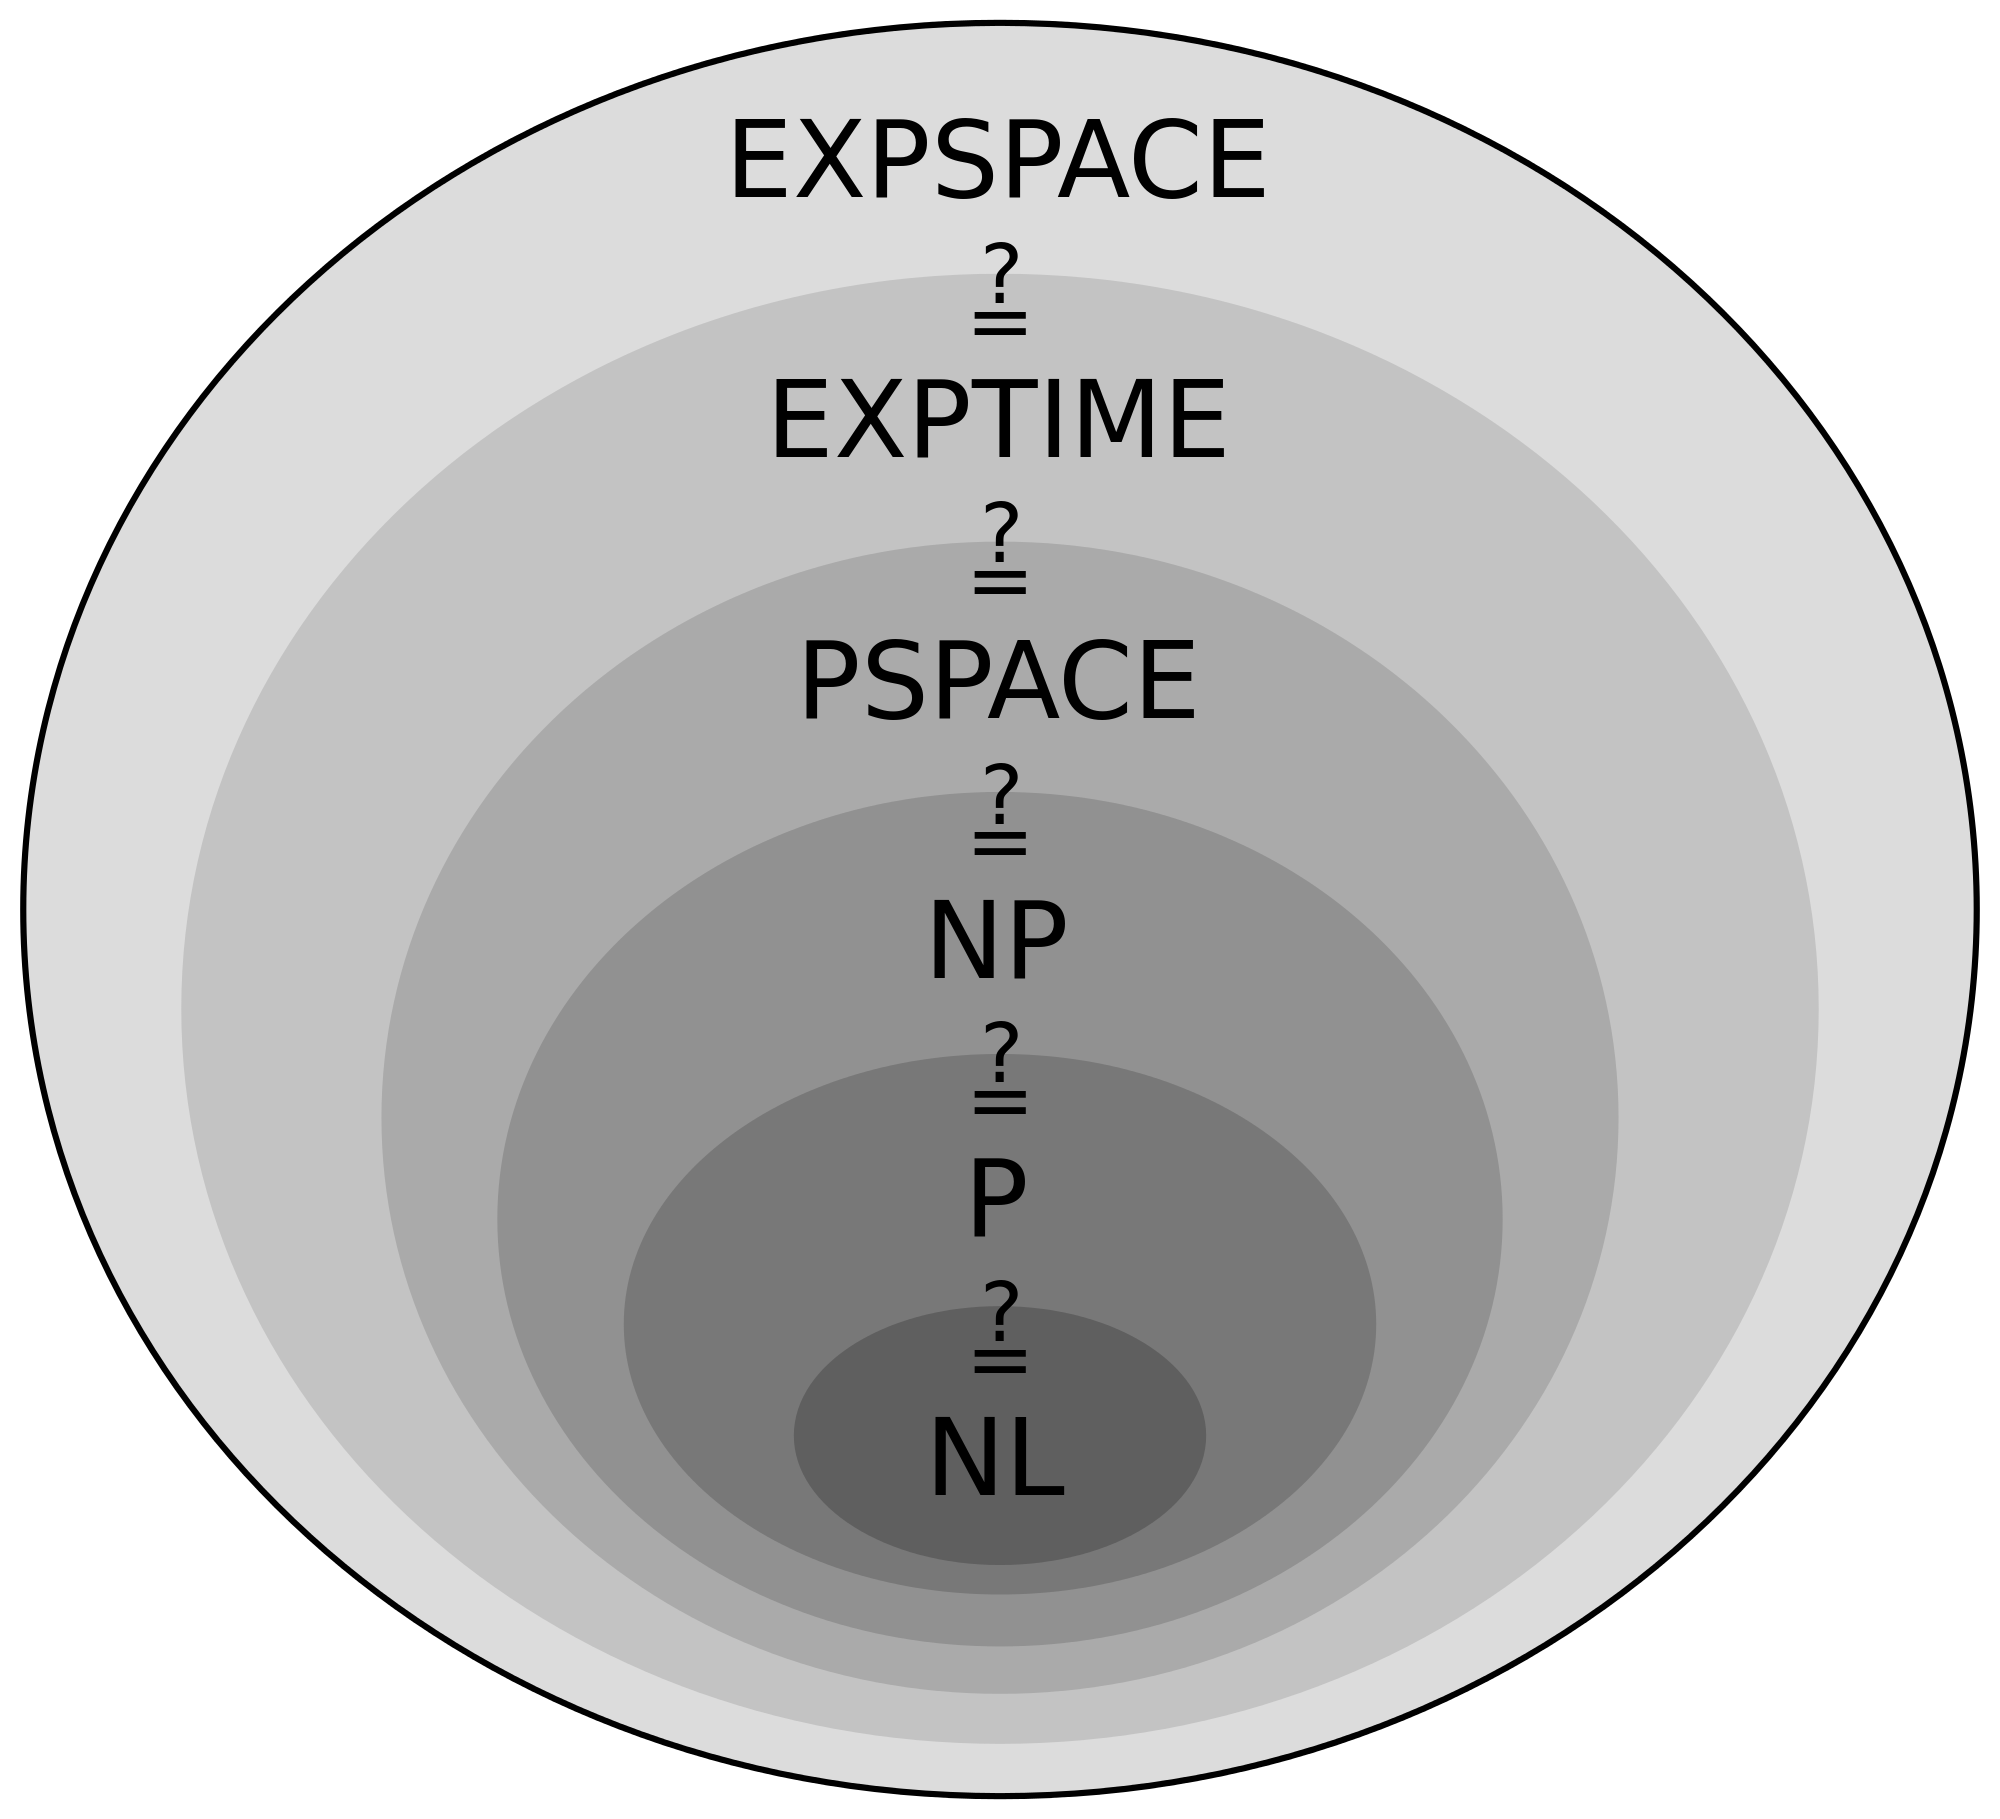
\includegraphics[width=\textwidth]{media/complexity.png}
  \end{center}
\end{frame}

\begin{frame}{The Class $\p$}
  
  A decision problem $D$ is in class $\p$ if there exists a BSS
  Machine $M$ and constants $c, q \in \reals$ such that:
  \begin{itemize}
  \item $M$ decides $D$
  \item For every $x \in D$, $\cost(\compute_M(x) < c \size(x)^d$.
  \end{itemize}
  
\end{frame}

\begin{frame}{Outline}
  \begin{center}
    \scaletopagewidth{\outlinefinal}
  \end{center}
\end{frame}

\begin{frame}{Verifiers}

  Recall our \subsum{} instance:

  \vspace{\baselineskip}

  $(\;\set{1,4,7,-5,-3,18,-6,12}\;, \;10\;)$

  \vspace{\baselineskip}

  The subset $\set{18, -3, -6, 1}$ is a short ``proof'' that this is a
  Yes Instance.

  \vspace{\baselineskip}

\end{frame}

\begin{frame}{Verifiers}

  A machine $M$ taking inputs $(x, w)$ is a \textbf{verifier} for a decision
  problem $D$ if:

  \begin{itemize}
  \item For all $x \in D$, there exists a $w$ such that $M$ accepts
    $(x, w)$ if and only if $x \in D_{yes}$
  \end{itemize}\pause

  A verifier for a problem $D$ is a machine that can use proofs to
  check if some $x$ belongs to $D_{yes}$.\pause

  \vspace{\baselineskip}

  In our example: $x = (\;\set{1,4,7,-5,-3,18,-6,12}\;, \;10\;)$ and
  $\set{18, -3, -6, 1}$.

\end{frame}

\begin{frame}{The Class $\np$}

  A problem $D$ is in class $\np$ if there exists a machine $M$ over
  $R$ and constants $c, q$ such that:

  \begin{itemize}
    \item M is a verifier for $D$.
    \item If $x \in D_{yes}$, then there exists a $w$ such that $M$
      accepts $(x, w)$ with $\cost(\compute_M(x, w)) \leq c
      size(x)^d$.
    \item If $x \notin D_{yes}$, no $w$ exists such that $M$ accepts
      $(x, w)$.
  \end{itemize}
  
\end{frame}

\begin{frame}{Nondeterministic Turing Machines}

  \begin{columns}

    \column{0.5\textwidth}
    Standard TM Transition:
    \functype{\delta}{(Q \times \Gamma)}{(Q \times \Gamma \times
      \set{\leftarrow, \rightarrow})}
       
    \column{0.5\textwidth}

    \begin{center}
      \detercomptm{}
    \end{center}
  \end{columns}
\end{frame}

\begin{frame}{Nondeterministic Turing Machines}

  \begin{columns}

    \column{0.5\textwidth}
    Nondeterministic TM Transition:
    \functype{\delta}{(Q \times \Gamma)}{\power{Q \times \Gamma \times
      \set{\leftarrow, \rightarrow}}}
       
    \column{0.5\textwidth}

    \begin{center}
      \scaletopagewidth{\ndetercomptm{}}
    \end{center}
  \end{columns}
\end{frame}

\begin{frame}{\ndet Machines}

  For standard BSS Machines, a branch node is defined by a pair
  $(\beta^+, \beta^-$, along with the branching function $h$.\pause

  \vspace{\baselineskip}

  \textbf{Idea:} Allow branch nodes to have multiple Yes and No nodes.\pause
  
  \vspace{\baselineskip}

  An \ndet Machine's branch nodes are defined by a branching function,
  plus two nonempty sets:

  $$\beta^+_\eta = \set{\yesnode{1}, \yesnode{2}, \ldots, \yesnode{i}}$$
  $$\beta_\eta^- = \set{\nonode{1}, \nonode{2}, \ldots, \nonode{j}}$$
\end{frame}

\begin{frame}{\ndet Computations}
  
\end{frame}

\end{document}